\documentclass[preprint,authoryear,11pt]{elsarticle}
\usepackage{amsmath,amssymb}
\usepackage{fullpage}
\usepackage{adjustbox}
\usepackage{setspace}
\usepackage[dvipsnames]{xcolor}
\usepackage{fixltx2e}

\usepackage{amsthm}
\usepackage [autostyle, english = american]{csquotes}
\MakeOuterQuote{"}
\usepackage{titlesec}
\usepackage{amsthm}
\usepackage{ragged2e}
\usepackage{setspace}
\usepackage[stable,bottom]{footmisc}
\usepackage{color}
\usepackage{graphicx}
\usepackage{graphics}
\usepackage{epstopdf}
\usepackage{siunitx}
\usepackage{dcolumn}




\usepackage[hidelinks]{hyperref}
\usepackage{units}
\hypersetup{
%    colorlinks=true,
    linktocpage=true,
    pdfstartpage=1,
    pdfstartview=FitH,
    breaklinks=true,
    pdfpagemode=UseNone,
    pageanchor=true,
    pdfpagemode=PageWdth,
    plainpages=true,
    bookmarksnumbered,
    bookmarksopen=false,
    bookmarksopenlevel=2,
    hypertexnames=true,
    pdfhighlight=/O,
    urlcolor=Black,
    linkcolor=Black,
    citecolor=Black,
    pdftitle={},
    pdfauthor={\textcopyright\ Kwong Yew Low (Rand)},
    pdfsubject={},%
    pdfkeywords={},%
    pdfcreator={pdfLaTeX},%
    pdfproducer={LaTeX with hyperref and classicthesis}%
}

\usepackage[all]{hypcap}

\titleformat{\subsubsection}[hang]{\normalfont\scshape}{\thesubsubsection}{3pt}{}
\titlespacing{\subsubsection}{0pt}{*2}{*2}
\usepackage{printlen}
\uselengthunit{in}
\usepackage{caption}
\usepackage{booktabs}
\usepackage{longtable}
\usepackage{tabularx}
\usepackage{nccmath}
\usepackage{multirow}
\usepackage{tikz}
\usepackage{threeparttable}
\usepackage{glossaries} % rand added 120411
\robustify{\gls}
\usepackage{etoolbox}

\makeglossary % rand added 120411
%\usepackage{float} % rand added 140411
\usepackage{subfig} % rand added 140411
\usepackage[english]{babel} % rand added 140411
\usepackage{graphicx} % rand added 140411
\usepackage{graphics} % rand added 140411
\usepackage{lscape}

\makeatletter
\def\ps@pprintTitle{
  \let\@oddhead\@empty
  \let\@evenhead\@empty
  \let\@oddfoot\@empty
  \let\@evenfoot\@oddfoot
}
\makeatother

\setcounter{topnumber}{2} \setcounter{bottomnumber}{2}
\setcounter{totalnumber}{4}
\renewcommand{\topfraction}{0.9}
\renewcommand{\bottomfraction}{0.8}
\renewcommand{\textfraction}{0.07}
\renewcommand{\floatpagefraction}{0.7}

\usetikzlibrary{snakes}
\usetikzlibrary{decorations}
\titlespacing*{\section}{0pt}{18pt plus 6pt minus 3pt}{9pt plus 6pt minus 3pt}
\titlespacing*{\subsection}{0pt}{12pt plus 6pt minus 3pt}{3pt plus 6pt minus 3pt}
\titlespacing*{\subsubsection}{0pt}{12pt plus 6pt minus 3pt}{3pt}
\interfootnotelinepenalty=10000
\linespread{1.05}
\newcommand{\tnl}{\tabularnewline}
\newcommand{\tab}{\hspace*{1em}}

\onehalfspacing
%\doublespacing

\newacronym{mvpt}{MVPT}{Mean-Variance Portfolio Theory}
\newacronym{asx}{ASX}{Australian Stock Exchange}
\newacronym{fso}{FSO}{Full Scale Optimization}
\newacronym{var}{VaR}{Value-at-Risk}
\newacronym{arma}{ARMA}{Autoregressive moving average}
\newacronym{rmse}{RMSE}{Root mean square error}
\newacronym{spa}{SPA}{Superior Predictive Ability}
\newacronym{cvar}{CVaR}{Conditional Value-at-Risk}
\newacronym{es}{ES}{Expected shortfall}
\newacronym{djia}{DJIA}{Dow Jones Industrial Average}
\newacronym{evt}{EVT}{Extreme Value Theory}
\newacronym{rs}{RS}{Regime Switching}
\newacronym{1/N}{$1/N$}{na\"{\i}ve equally-weighted}
\newacronym{ceq}{CEQ}{Certainty Equivalent Return}
\newacronym{garch}{GARCH}{GARCH}
\newacronym{garch-gjr}{GARCH-GJR}{GARCH-GJR}
\newacronym{crra}{CRRA}{Constant Relative Risk Aversion}
\newacronym{cava}{CAVA}{Canonical Autoregressive Vine Copulas}
\newacronym{dcc}{DCC}{Dynamic Conditional Correlation}
\newacronym{capm}{CAPM}{capital asset pricing model}
\newacronym{gjr-GARCH}{GJR-GARCH}{Glosten-Jagannathan-Runkle GARCH}
\newacronym{icapm}{ICAPM}{international capital asset pricing model}
\newacronym{swarch}{SWARCH}{Switching ARCH}
\newacronym{garchm}{GARCH-M}{Generalized AutoRegressive Conditional Heteroskedasticity in Mean}
\newacronym{mppm}{MPPM}{Manipulation-Proof Performance Measure}
\newacronym{xao}{XAO}{S&P/ASX All Ordinaries}
\newacronym{xpj}{XPJ}{S&P/ASX 200 A-REIT}
\newacronym{xdj}{XDJ}{S&P/ASX 200 Consumer Discretionary}
\newacronym{xsj}{XSJ}{S&P/ASX 200 Consumer Staples}
\newacronym{xej}{XEJ}{S&P/ASX 200 Energy sector}
\newacronym{xxj}{XXJ}{S&P/ASX 200 Financials-x-A-REIT}
\newacronym{xfj}{XFJ}{S&P/ASX 200 Financials}
\newacronym{xhj}{XHJ}{S&P/ASX 200 Health Care}
\newacronym{xnj}{XNJ}{S&P/ASX 200 Industrials}
\newacronym{xij}{XIJ}{S&P/ASX 200 Information Technology}
\newacronym{xmj}{XMJ}{S&P/ASX 200 Materials}
\newacronym{xtj}{XTJ}{S&P/ASX 200 Telecom. Services}
\newacronym{xuj}{XUJ}{S&P/ASX 200 Utilities}
\newacronym{gics}{GICS}{Global Industry Classification Standard}
\newacronym{caviar}{CAViaR}{Conditional Autoregressive Value at
Risk by Regression Quantiles}
\newacronym{nber}{NBER}{National Bureau of Economic Research}
\newacronym{ftse}{FTSE}{Financial Times Stock Exchange}
\newacronym{cara}{CARA}{Constant absolute risk aversion}
\newacronym{mvn}{MVN}{multivariate normality}
\newacronym{cvc}{CVC}{canonical vine copula}
\newacronym{sc}{SC}{standard copula}
\newacronym{mv}{MV}{mean-variance}
\newacronym{cdf}{CDF}{cumulative distribution function}
\newacronym{pdf}{pdf}{probability distribution function}

\newacronym{vcv}{VCV}{variance-covariance}
\newacronym{skew-t}{Skew-T}{Skewed Student $t$}
\newacronym{ifm}{IFM}{inference for margins}
\newacronym{dm4}{DM4}{4-factor data-and-model }
\newacronym{dm3}{DM3}{3-factor data-and-model }
\newacronym{dm1}{DM1}{1-factor data-and-model }
\newacronym{etf}{ETF}{exchange traded funds}
\newacronym{mle}{MLE}{Maximum Likelihood Estimator}
\newacronym{ew-rebal}{EWR}{$1/N$ with rebalancing}
\newacronym{ew-no-rebal}{EWNR}{$1/N$ without rebalancing}
\newacronym{mv-in-samp}{MVIS}{in-sample mean-variance}
\newacronym{mv-s}{MVS}{sample-based mean-variance}
\newacronym{bs-diff}{BSD}{Bayesian diffuse-prior}
\newacronym{bs}{BS}{Bayes-Stein}
\newacronym{dm}{DM}{Bayesian Data-and-Model}
\newacronym{min}{MIN}{minimum-variance}
\newacronym{mp}{MP}{\citet{mackinlay2000} missing-factor model}
\newacronym{mv-c}{MVC}{sample-based mean-variance with shortsale constraints}
\newacronym{mv-tz}{MVTZ}{sample-based mean \& adjusted \gls{vcv} developed by \citet{tu2011}}
\newacronym{bs-c}{BSC}{Bayes-Stein with shortsale constraints}
\newacronym{min-c}{MINC}{minimum-variance with shortsale constraints}
\newacronym{g-min-c}{GMINC}{minimum-variance with generalized constraints}
\newacronym{mv-min}{MVMIN}{\citet{kan2007} `three-fund' model}
\newacronym{ew-min}{EWMIN}{mixture of minimum-variance and $1/N$}
\newacronym{ew-mv}{EWMV}{combination of $1/N$ and \citet{markowitz1952}}
\newacronym{ew-kz}{EWKZ}{combination of $1/N$ and \citet{kan2007}}


\usepackage{array,booktabs}
\usepackage{tabularx}
\usepackage{booktabs}
\setlength{\extrarowheight}{7.5pt}
\usepackage{amsmath}
\usepackage{natbib}
\usepackage{dcolumn}
\newcolumntype{d}[1]{D{.}{.}{#1}}
\usepackage[labelfont=bf]{caption}
\captionsetup{labelsep=space,justification=justified,singlelinecheck=off}
\renewcommand{\figurename}{Fig.}
\addto\captionsenglish{\renewcommand{\figurename}{Fig.}}

\makeatletter
\def\@seccntformat#1{%
	\expandafter\ifx\csname c@#1\endcsname\c@section\else
	\csname the#1\endcsname\quad
	\fi}
\makeatother
%----------------------------------------------------------------------------------------
\begin{document}
\begin{frontmatter}
\title{More than jewelry\tnoteref{t1}}
\tnotetext[t1]{Acknowledge any grants received, anyone who has helped you on
the paper or anywhere you have presented your work}





\author[uqbs1]{Yiran Yao\corref{cor1}}\ead{Author@university.edu.au}
\author[uqbs1]{Rand Low}%\ead{r.faff@business.uq.edu.au}
\author[ncc]{Robert Faff}%\ead{kjersti@nr.no}


\address[uqbs1]{UQ Business School, University of Queensland, Brisbane, 4072, Australia}
\address[ncc]{Another University}


\cortext[cor1]{Principal corresponding author}

%\fntext[fn1]{Author footnote}
%\fntext[fn2]{Another author footnote}
%\fntext[fn3]{Yet Another author footnote}

\begin{abstract}
As gold has been thoroughly studied as an investment, this paper also explores into other precious metals such as silver, platinum, and palladium, with the addition of diamonds. We examine their properties against the US market as well as Australian market. Using daily data from Aug 1993 to Aug 2013, 


\end{abstract}




\begin{keyword}
Safe haven \sep Hedging \sep Copula \sep Precious metals \sep Diamonds  \\
\emph{JEL classification}: G??, C?? \\
\end{keyword}

\end{frontmatter}


%----------------------------------------------------------------------------------------
%	Introduction
%----------------------------------------------------------------------------------------
\newpage
\section{1. Introduction}
\label{sec:introduction} \glsresetall

\noindent With an effort to fight against the market volatilities, hence entered alternative investments with their appealing characteristics of low volatilities with the market. More investors have come to the realization of the value of precious metals and gems, not only as jewelry, but also as assets that preserves their value during adverse market conditions. While gold has long been a popular topic in the investment world, other physical assets such as platinum and diamonds hae gradually shined their way into the spotlight. This paper will be examining the reaction of gold, silver, platinum, palladium and additionally diamonds to fluctuations in the market, more specifically whether they act like hedges or safe havens, by two distinct methods.
\newline\newline
\noindent Historically gold prices seem to fluctuate negatively against the market. In response to downgrading of US's credit ratings \citet{2011}, the price of gold skyrocketed to approximately \$1900/ounce while the US market experienced a 16.7\% drop. A reverse situation occurred recently, where gold saw a largest decline in price in 32 years as investors shy away \citet{keylist}, as a vast contrast the market continued its course of rising.
\newline\newline
\noindent A number of previous studies have examined the particular role of gold among investments, whether and when it is a hedge or a safe haven. \citet{mccown_is_2006} demonstrate gold's zero-beta property by estimating capital asset pricing model, with evidence shown for its inflation-hedging ability. With regard to stock markets, \citet{baur_is_2009}, \citet{baur_is_2010} found that gold acted as a safe haven against stock markets, although conditions varied for different markets. The results were further verified by \citet{joy_gold_2011}, where the conclusion is made that in times of market stress, no evidence was discovered to suggest that the safe haven status were effective. According to the research by \citet{pullen_comparative_2011}, the hedging ability exhibited by gold bullion is clear and strong. By analyzing both data from the US and the UK market,\citet{ciner_hedges_2013} suggest the hedging role of gold against exchange rate fluctuations. Evidence found by \citet{reboredo_is_2013}, \citet{joy_gold_2011}, \citet{capie_gold_2005} support the result that gold can act as a hedge against movements in USD. \citet{pukthuanthong_gold_2011} extend the research to other currencies and find that US dollars is not the only currency that gold is negatively associated to, the same relationship also applies to Euro, Yen, and Pound.
\newline\newline
\noindent Apart from gold, other precious metals including platinum and silver have also been found to possess the ability to play the role as diversifiers in portfolios and exhibit hedging capability especially during periods of high market volatility. Among all three metals being studied, gold proved to be the optimal choice for hybrid portfolio, offering the most efficiency gains \citep{hillier_precious_2006}. \citet{conover_can_2009} conclude that improvements in portfolio performance can be achieved by either investing directly or indirectly in precious metals, and effects are found to be more prominent with indirect investments. Again gold claims the winner in diversifying and hedging against inflation pressure. In the research carried out by \citet{lucey_what_2013}, through the analysis of quarterly data evidence suggests that at certain times silver, platinum and palladium can act as safe haven when gold does not, and the effect can sometimes be stronger. \citet{hood_is_2013} argue that unlike gold, platinum and silver act as neither hedge nor safe haven for the US stock market. Gold on the other hand, while serving as a hedge and a weak safe haven, does not exhibit negative correlation with the market during periods of extreme conditions. Among the four metals \citet{sari_dynamics_2010} confirm that platinum and palladium are closely related, rising platinum prices may act as a precursor for a price increase in palladium. A further investigation into their relationships by \citet{sensoy_dynamic_2013} draw the conclusion that since the correlation among those metals have increase drastically and the trend is likely to be preserved, precious metals may be classified as a single asset in the future. Gold, being used as a popular investment choice and international reserve currency, exert uni-directional volatility shift contagion effect on all precious metals. The study into silver displays a similar effect on platinum and palladium.
\newline\newline
\noindent As for gems, there exists a well-known tag line in the world of jewelries --- A diamond is forever. Diamond consumption has escalated in the past few decades. Looking into the US market alone, currently diamonds totaled 49\% of all jewelry purchases \citet{webpage}. Prior to 2000, the majority of the rough diamonds were dominated by one company, De Beers, a giant that controlled a proportion of diamond sales as high as 80\% \citet{webpage}. With declining production in gem quality diamonds, absence of significant discoveries of diamond deposits in recent years, along with rising demand in both traditional and emerging countries, particularly in China, a change is preceived to take place in the diamond market \citet{webpage}. An annual report from Bain \& Company \citet{bain2013} points out that supply of diamond will grow at a rate sufficiently to meet demand until 2016. However the subsequent declining supply will widen the demand-supply gap through early 2020s.
\newline\newline
\noindent There are few paper examining the quality of diamonds as an investment and its diversification potential. \citet{auer_diamonds_2013} conclude that diversified portfolios that solely composed of stocks when stock markets are weak. Low time-varying correlations to traditional assets provide indications of their diversifying qualities, yet the potential can only be reached with rather high proportion of diamond in the portfolio. \citet{renneboog_hard_2012} find evidence of relatively superior performance of diamonds than stock market. When comparing diamond to traditional metals, \citet{auer_could_2014} state that the investment performance of diamonds is lower than the one of gold and silver, and within the US market diamonds have only acted as a weak hedge and a weak safe haven against stock market downturns and currency risk associated with the US dollar. In terms of the characteristics of the entire market, \citet{chong_long-range_2012} note that diamond daily returns do not have long memory, yet the existence of long memory is found to be present in volatilities. 
\newline\newline
\noindent Our paper aims to investigate the hedge or safe haven status of all major precious metals and extending to precious gems.


%----------------------------------------------------------------------------------------
%	Data
%----------------------------------------------------------------------------------------
\section{2. Data}
\label{sec:data}
\noindent The data set consists of daily returns of four precious gems (gold, silver, platinum and palladium), four precious gems (diamond, ruby, emerald and sapphire), and S\&P 500 index. All data is gathered from Datastream. Metal data covers a period from Aug 2, 1993 to Aug 2, 2013, a sample size of 5219 observations, and a shorter period for diamond data starting from Aug 2, 2004 to the same end date, totaled 2349 observations. The sample period encompasses Asian crisis in 1997, crash of Dotcom bubble in 2001, global financial crisis in 2008-09 and more recently the downgrade of US credit ratings in 2011. PolishedPrices diamond price indicies categorizes diamond indicies into three categories, commercial index, fine index and mixed index. Each index is further broken down into three subcategories based on weight of diamonds: 1 carat, 0.5 carat and 0.3 carat. Additionally there is an overall index that tracks the price movements of all diamonds that are contained in these nine indicies. Table \ref{tab:data_descrip}  exhibits descriptive statistics of all data included. Through inspecting the correlation with the S\&P 500, gold is found to be the only metal that negatively correlated with the S\&P 500. Palladium on the other hand shows the highest correlation with the market. 

\begin{table}[htp!]
	\caption{\newline Descriptive statistics of all asset returns and all index returns in US dollar.}
	\label{tab:data_descrip}
	\renewcommand\arraystretch{0.7}
	\begin{tabularx}{\linewidth}{>{\arraybackslash\small}X *{5}{>{\raggedleft\arraybackslash\small}m{.08\linewidth}}
			@{\hspace{1em}}
			*{3}{>{\raggedleft\arraybackslash\small}m{.08\linewidth}}}
		\hline
		  & \multicolumn{5}{c}{Assets}   & \multicolumn{3}{c}{Indicies} \\
		\cmidrule(r{1em}){2-6} \cmidrule{7-9}
		       &  Diamond  & Au  & Ag & Pt & Pd & World & US & Australia \\
		\hline
		  Mean &  0.009\%  & 0.023\%   &  0.025\%  &  0.024\%  & 0.031\%   & 0.019\%  &  0.026\% & 0.020\%   \\
		  Std  &  1.269\%  & 1.814\%   &  1.418\%  &  2.140\%  & 1.028\%   & 0.981\%  &  1.194\% &	0.971\%  \\
		  Max  &  13.245\% & 7.382\%   &  13.665\% & 11.728\%  & 15.841\%  & 9.097\%  & 10.957\% & 5.724\%   \\
		  Min  & -12.867\% & -10.162\% & -12.982\% & -17.277\% & -17.859\% & -7.325\% & -9.470\% & -8.704\%  \\
		  Skew & 0.451     & -0.374    & -0.568    & -0.673    & -0.157    & -0.368   & -0.243   & -0.471    \\
		  Kurt & 18.571    & 7.709     & 6.138     & 10.630    & 6.504     & 8.037    & 8.663    & 6.079     \\
		  Corr. US & & & & & & & & \\
		\hline  
		
		\bottomrule
	\end{tabularx}
	\caption*{\newline Notes: 5219 daily return data from Aug 2, 1993 to Aug 2, 2013. }
\end{table}

\noindent Fig.~\ref{fig:metal_sp500} displays the evolution of all four precious metal prices against S\&P 500 index during the time interval being studied, and Fig. \ref{fig:diamond_sp500} shows the trend of diamond prices. Among all four metals it is obvious that silver sees most volatile fluctuations, especially after global financial crisis. Both platinum and silver experienced significant shift in price during the time. A closer look to the crisis period suggests that silver and platinum soared in the early stage and subsequently took a plunge as the situation worsened. The recovery of the three metal prices started at the end of 2008, eventually moved in the opposite direction against the market. As the market picked up its upward trend since 2013, the metals in study all underwent a continuous decline in prices. It can be observed from the graph that palladium remained relatively stable compared to its counterparts. Fig. \ref{fig:convol_metal} demonstrates the time-varying volatility of metal return series estimated with a GARCH(1,1) model.

\begin{figure}
	\centering
	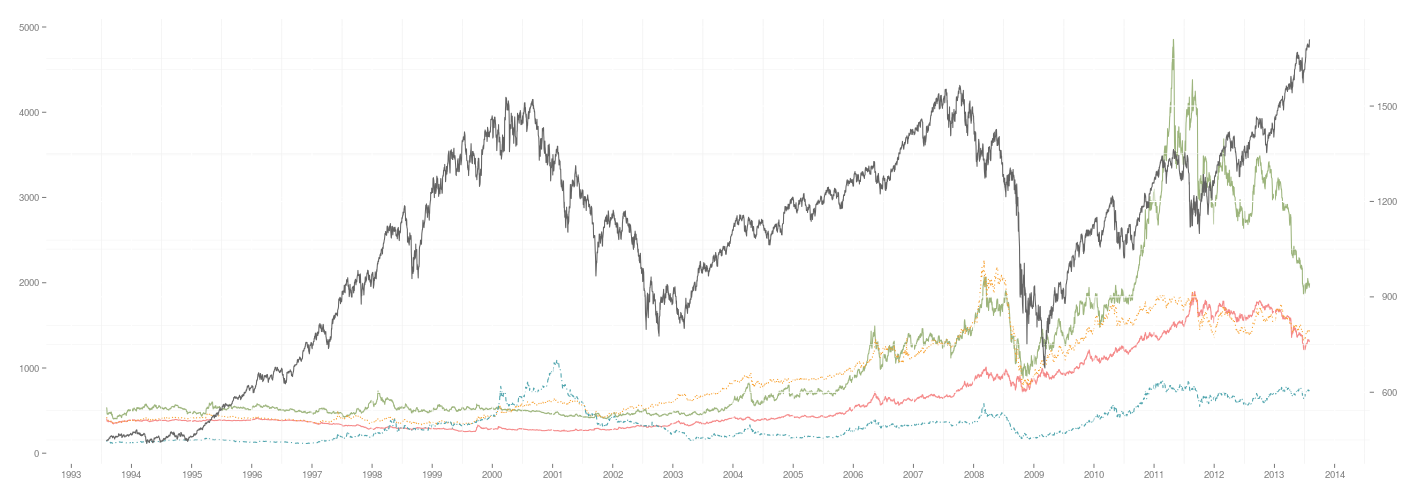
\includegraphics[scale=0.3]{metal_prices}
	\caption{Evolution of prices of four precious metals. Silver price is showed in a different unit (cent per troy ounce) than gold, platinum and palladium (dollar per troy ounce). The S\&P 500 index is measured on the right vertical axis while metal prices are measured on the left vertical axis. The figure exhibits data spanning the entire sample period from Aug 2, 1993 to Aug 2, 2013.}   %PLOTTING NEEDS TO BE CHANGED
	\label{fig:metal_sp500}
\end{figure}

\begin{figure}
	\centering
%	\includegraphics[scale=0.3]{diamond_sp500}
	\caption{Evolution of prices of diamond price indicies. The S\&P 500 index is measured on the left vertical axis while diamond index is measured on the right vertical axis. The figure exhibits data spanning the entire sample period of diamonds from Aug 2, 2003 to Aug 2, 2013.}
	\label{fig:diamond_sp500}
\end{figure}

\begin{figure}
	\centering
	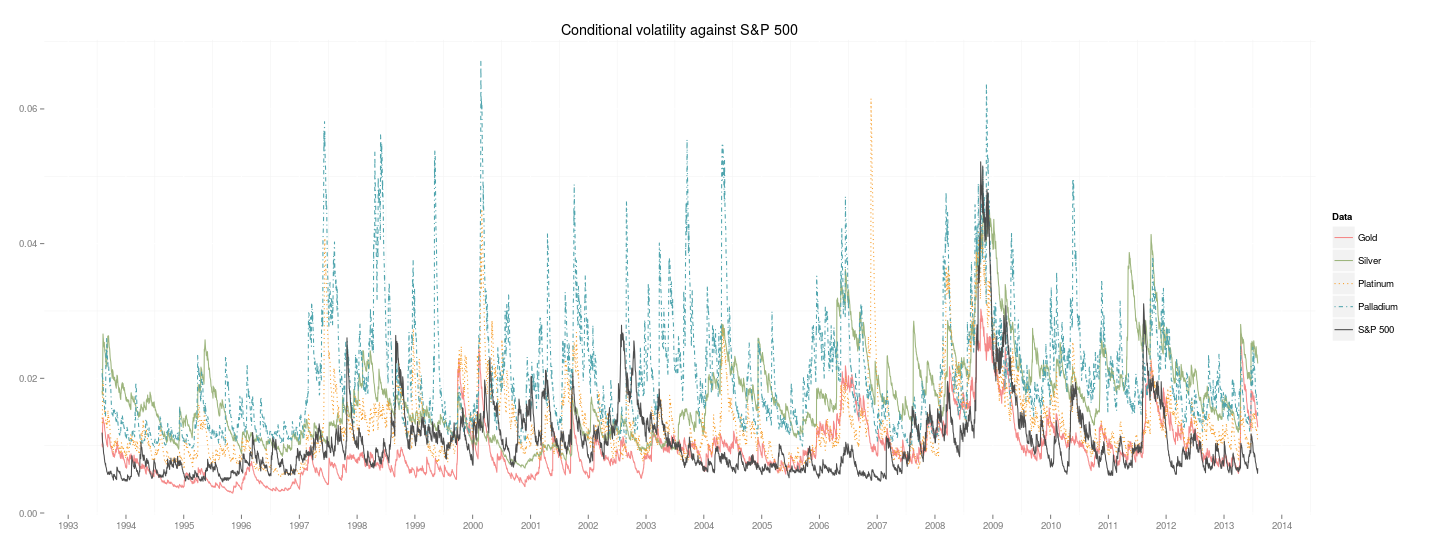
\includegraphics[scale=0.34]{sp500Plot}
	\caption{Daily conditional volatility (GARCH(1,1) estimates) of the S\&P 500 index return and the return on all assets over a period from Aug 2, 1993 to Aug 2, 2013. }
	\label{fig:sp500Plot}
\end{figure}


%----------------------------------------------------------------------------------------
%	Methods
%----------------------------------------------------------------------------------------
\section{3. Research methods}
\label{sec:methods}
\noindent The initial stage of the analysis utilizes the following model which was first proposed and used by \citet{baur_is_2010}, specifies as follows:

\begin{align}
	 r_{asset,t} &= a + b_{t}r_{stock,t} + \varepsilon_{t} \label{eq:mean_equation}\\
	 b_{t} &= c_{0} + c_{1}D(r_{stock}q_{10}) + c_{2}D(r_{stock}q_{5}) + c_{3}D(r_{stock}q_{1}) \label{eq:bt}\\
	 h_{t} &= \omega + \alpha\varepsilon_{t-1}^2 + \beta h_{t-1} \label{eq:garch11}
\end{align}

\noindent Equation \eqref{eq:mean_equation} models the relation of each metal (gem) and stock returns. The parameters to estimate are α and bt. The error term is et. bt is modeled as a dynamic process given by Equation \eqref{eq:bt}. The parameters to estimate in Equation \eqref{eq:bt} are $c_{0}$, $c_{1}$, $c_{2}$ and $c_{3}$. D(...) are dummy variables to capture extreme stock market movements and evaluate to one if stock market return at time t exceeds a certain threshold given by the 10\%, 5\% and 1\% quantile of the return distribution, and zero otherwise. The residual term $e_{t}$ is modeled as a GARCH(1,1) process to account for heteroscedasticity in the data. All equations are jointly estimated with Maximum Likelihood methods. If one of the parameters $c_{1}$, $c_{2}$ or $c_{3}$ is significantly different from zero, then this suggests relationship between the asset in question and the stock market. If the parameters in Equation \eqref{eq:bt} are non-positive, the asset acts as a weak safe haven. If the parameters are negative and statistically different from zero, the asset becomes a strong safe haven. In the event of parameter $c_{0}$ equals zero or negative, and the sum of the parameters $c_{1}$ to $c_{3}$ are not jointly positive exceeding the value of $c_{0}$, the asset serves as a hedge, where negative $c_{0}$ suggests strong hedge and a value of zero indicates weak hedge. \newline
\noindent Choosing the conditional volatility of the world portfolio as a proxy for uncertainty, we can change the model under the assumption that as the uncertainty of the market changes, the asset-stock relation also varies. If the conditional volatility of the world index is estimated with a GARCH process and different volatility levels are chose, an alternative to \eqref{eq:bt} can be specified as follows
\begin{align}
	b_{t} = c_{0} + c_{1}D(h_{world}q_{90,t-1}) + c_{2}D(h_{world}q_{95,t-1}) + c_{3}D(h_{world}q_{99,t-1}) \label{eq:vol}
\end{align}
where the dummy variable is equal to one if the lagged conditional volatility of the world index exceeds the 90\% (95\% and 99\%) quantile and zero otherwise. \newline
\noindent Finally we break down the entire study period and identify certain periods such as economic or financial crises. Time dummies are equal to one if the returns fall within the predefined period and zero otherwise. The model would be specified as follows
\begin{align}
	 b_{t} = c_{0} + c_{1}D(\text{Asian Crisis, 1997}) + c_{2}D(\text{GFC, 2008}) + c_{3}(\text{US credit downrating, 2011}) \label{eq:crisis}
\end{align}
\noindent If the parameters $c_{1}$, $c_{2}$ or $c_{3}$ are zero or negative, the asset is a safe haven in the respective crisis period. On the other hand a positive parameter means that the asset co-moves with the market and is not a safe haven. \newline
\noindent The next section presents the estimation results and the analysis of figures.


%----------------------------------------------------------------------------------------
%	Results
%----------------------------------------------------------------------------------------
\section{4. Empirical results}
\label{sec:results}
Estimated results of the regression model given by Equations \eqref{eq:mean_equation}, \eqref{eq:bt}, and \eqref{eq:garch11} are reported in Table \ref{tab:eq123_results}. The table contains the estimates of $c_{0}$ and the total effects for extreme market conditions, which is the sum of $c_{0}$ and $c_{1}$ for the 10\% quantile, the sum of $c_{0}$, $c_{1}$, and $c_{2}$ for the 5\% quantile, and the sum of $c_{0}$, $c_{1}$, $c_{2}$ and $c_{3}$ for the 1\% quantile.
\newline\newline
\noindent An examination of the hedge column shows that only gold serves as a hedge against the US stock market. All other assets possess significant positive correlation with the S\&P 500 with palladium being the highest. It is also showed that gold is a strong safe haven at 10\% as well as 1\% quantiles. Silver, platinum, and palladium on the other hand, do not act as safe havens. All three metals exhibit strong positive correlation with the S\&P 500 at any quantile. Diamond, while not being a hedge against the market, negatively correlated with the index at 10\% quantile, suggesting that it is a strong safe haven at the level. The Australian market has negative correlation with all four metals at the lowest quantile, additionally both platinum and diamonds are safe haven to the market at the 5\% quantile.
\newline\newline
\noindent Table \ref{tab:volatility_results} presents the estimation results of model specified in \eqref{eq:vol}. We choose to study with extreme high volatilities given by the daily conditional volatility of the world index estimated with a GARCH(1,1) process. Three levels of volatility are chosen as a proxy for global financial market uncertainty. As the results shown, none of the asset except gold is a hedge against the US market. Apart from the hedging ability it also act as safe haven in periods of volatility surpassing 90\% and 95\%, but not 99\%. Silver and Platinum both work as safe haven when volatility is greater than 95\%. For the Australian market gold and diamonds are safe havens at 90\% volatility threshold. Interestingly enough, in periods of extreme volatility (99\% threshold), diamonds become the only asset that hold the safe haven potential.
\begin{table}[htp!]
	\caption{\newline The table presents the estimation results for the role of gold, silver, platinum, palladium, and diamond as a hedge and a safe haven asset for daily returns. The sample period is from Aug 2, 1993 to Aug 2, 2013 for all metals and Aug 2, 2004 to Aug 2, 2013 for diamonds. Panel A, B, and C represent results against World index, S\&P 500 Composite index, and ASX 200 index respectively. Negative coefficients in the hedge column signifies that the asset is a hedge against stocks. Zero (negative) coefficients in extreme market conditions (quantile 10\%, 5\%, and 1\%) indicate that the asset is a weak (strong) safe haven.}
	\label{tab:eq123_results}
	\renewcommand\arraystretch{0.65}
	\begin{tabularx}{\linewidth}{*{2}{>{\arraybackslash\small}p{.14\linewidth}}
			                     *{4}{>{\arraybackslash\small}p{.14\linewidth}}S[table-format=1.3]}
		\hline
		\multicolumn{6}{c}{Australia} \\
		\hline
		      &     & \multirow{2}{*}{Hedge}  & \multicolumn{3}{c}{Safe haven quantiles} \\
		\cmidrule{4-6}
		      &    &        & 10\% & 5\% & 1\% \\
		\hline
		\multirow{5}{*}{Metals} & Gold  & 0.125 & 0.091 & -0.030 & -0.236*** \\
		                            & Silver & 0.306 & 0.144 & -0.046 & -0.243** \\
		                            & Platinum & 0.339 & 0.083 & 0.104 & -0.154** \\
		                            & Palladium & 0.339 & 0.040 & 0.062 & -0.207*** \\
		                            & Rhodium & -0.022 & 0.082 & -0.001 & -0.172*** \\
		\hline
		\multirow{8}{*}{Diamonds} & 1ct Comm. & 0.092 & 0.106 & -0.040 & -0.247 \\
		                          & 1ct Fine & 0.045 & 0.00 & -0.252 & 0.198 \\
		                          & 0.5ct Comm. & -0.111 & 0.243 & -0.155 & -0.020 \\
		                          & 0.5ct Fine & -0.062 & 0.460 & -0.305 & -0.268 \\
		                          & 0.3ct Comm. & -0.029 & 0.064 & 0.068 & -0.186* \\
		                          & 0.3ct Fine & -0.075 & -0.042 & 0.282 & -0.353 \\
		                          & 3ct D Flawless & -0.723*** & 1.099 & -0.056 & 0.782 \\
		                          & 1ct D Flawless & -0.071 & 0.066 & 2.801 & -2.852*** \\
		\hline
	\end{tabularx}
\end{table}

\begin{table}[htp!]
	\caption{\newline }
	\renewcommand\arraystretch{0.65}
	\begin{tabularx}{\linewidth}{*{6}{>{\raggedleft\arraybackslash\small}p{.14\linewidth}}S[table-format=1.3]}
		\hline
		\multicolumn{6}{c}{China} \\
		\hline
		&     & \multirow{2}{*}{Hedge}  & \multicolumn{3}{c}{Safe haven quantiles} \\
		\cmidrule{4-6}
		&    &        & 10\% & 5\% & 1\% \\                      
		\hline
	    \multirow{5}{*}{Metals}  & Gold       & 0.113 & -0.036  & 0.039 & -0.007 \\
                                     & Silver     & 0.230 & -0.112  & 0.180 & -0.022 \\
		                             & Platinum   & 0.224 & 0.002 & -0.017 & -0.011 \\
		                             & Palladium  & 0.255 & 0.037 & 0.031 & -0.045 \\
		                             & Rhodium    & -0.003 & -0.018 & 0.015 & 0.017 \\
		\hline
		\multirow{8}{*}{Diamonds} & 1ct Comm. & -0.007 & 0.00 & 0.061 & -0.037 \\
		                          & 1ct Fine & 0.025 & -0.101 & 0.076 & 0.126 \\
		                          & 0.5ct Comm. & -0.11 & -0.133 & 0.116 & 0.064 \\
		                          & 0.5ct Fine & 0.061 & -0.171 & 0.057 & 0.108 \\
		                          & 0.3ct Comm. & -0.010 & -0.043 & 0.065 & -0.017 \\
		                          & 3ct D Flawless & -0.021 & 0.193 & -0.174 & 0.008 \\
		                          & 1ct D Flawless & 0.007 & -0.767*** & 0.736 & 0.124 \\
		\hline
	\end{tabularx}
	\caption*{\newline
		      *   Statistical significance at the 10\% level.\\
		      **  Statistical significance at the 5\% level.\\
		      *** Statistical significance at the 1\% level.}
\end{table}
\begin{table}[htp!]
	\caption{\newline }
	\renewcommand\arraystretch{0.65}
	\begin{tabularx}{\linewidth}{*{6}{>{\raggedleft\arraybackslash\small}p{.14\linewidth}}S[table-format=1.3]}
		\hline
		\multicolumn{6}{c}{Pacific} \\
		\hline
		&     & \multirow{2}{*}{Hedge}  & \multicolumn{3}{c}{Safe haven quantiles} \\
		\cmidrule{4-6}
		&    &        & 10\% & 5\% & 1\% \\
		\hline
		\mu\\\\\\\\\\\][\'\'
		
		
		
		
		
		\']
		 `1QA2WS3ED4RF5ltirow{5}{*}{Metals} & Gold & 0.301 & -0.033 & -0.147** & 0.034 \\
		                            & Silver & 0.470 & 0.055 & -0.159 & -0.012 \\
		                            & Platinum & 0.331 & -0.033 & -0.015 & 0.024 \\
		                            & Palladium & 0.493 & 0.016 & -0.087 & 0.235 \\
		                            & Rhodium & -0.025 & 0.012 & 0.014 & -0.032\\
		\hline
		\multirow{8}{*}{Diamonds} & 1ct Comm. & 0.001 & 0.066 & -0.183 & 0.206 \\
		                          & 1ct Fine & 0.041 & 0.018 & -0.231 & 0.182 \\
		                          & 0.5 Comm. & -0.048 & -0.004 & -0.030 & 0.106 \\
		                          & 0.5 Fine & 0.037 & -0.039 & 0.021 & 0.015 \\
		                          & 0.3 Comm. & 0.004 & -0.096 & 0.092 & 0.036 \\
		                          & 0.3 Fine & -0.059 & 0.219 & -0.236 & 0.121 \\
		                          & 3ct D Flawless & -0.015 & 0.036 & 0.208 & -0.219 \\
		                          & 1ct D Flawless & -0.034 & 0.149 & -1.017*** & 0.902 \\
		\hline
	\end{tabularx}
	\caption*{\newline
	*   Statistical significance at the 10\% level.\\
	**  Statistical significance at the 5\% level.\\
	*** Statistical significance at the 1\% level.}
\end{table}

\begin{table}[htp!]
	\caption{\newline The table presents the estimation results for the role of assets as hedges and safe havens in period of increased volatility as a proxy for uncertainty. Negative coefficients imply that the asset is a hedge on average or a safe haven in periods of increased or extreme volatility. The total effect (Ttl. eff.) is the sum of the hedge coefficient ($c_{0}$) and the marginal effect ($c_{1}$, $c_{2}$, and $c_{3}$). The t-stats refer to the marginal effect.}
	\label{tab:volatility_results}
	\renewcommand\arraystretch{0.55}
	\begin{tabularx}{\linewidth}{>{\arraybackslash\small}p{2.3cm}
			*{2}{>{\raggedleft\arraybackslash\small}p{.08\linewidth}}
			@{\hspace{1em}}
			*{2}{>{\raggedleft\arraybackslash\small}p{.08\linewidth}}
			@{\hspace{1em}}
			*{2}{>{\raggedleft\arraybackslash\small}p{.08\linewidth}}
			@{\hspace{1em}}
			*{2}{>{\raggedleft\arraybackslash\small}p{.08\linewidth}}}
		\hline
		\multicolumn{9}{c}{Australia} \\
		\hline
		& \multicolumn{2}{c}{Hedge} & \multicolumn{2}{c}{Volatility\textgreater 90\%} & \multicolumn{2}{c}{Volatility\textgreater 95\%} &  \multicolumn{2}{c}{Volatility\textgreater 99\%} \\
		\cmidrule(r{0.8em}){2-3} \cmidrule(r{0.8em}){4-5} \cmidrule(r{0.8em}){6-7} \cmidrule{8-9}
		& Coeff. & t-stats & Ttl. eff. & t-stats & Ttl. eff. & t-stats & Ttl. eff. & t-stats \\
		\hline
		\multicolumn{9}{c}{Metals} \\
		\hline
			Gold &  &  &  &  &  &  &  &  \\
			Silver &  &  &  &  &  &  &  &  \\
			Platinum &  &  &  &  &  &  &  &  \\
			Palladium &  &  &  &  &  &  &  &  \\
			Rhodium &  &  &  &  &  &  &  &  \\
		\hline
		\multicolumn{9}{c}{Diamonds} \\
		\hline
		1ct Comm. & 0.10 & 1.67 & -0.05 & -0.90 & 0.35 & 1.24 & -0.30 & -0.97 \\
		1ct Fine & 0.03 & 0.42 & -0.11 & -0.62 & -0.02 & -0.16 & 0.28 & 0.65 \\
		0.5ct Comm. & -0.04 & -0.60 & -0.08 & -0.27 & -0.17 & -0.88 & 0.16 & 0.86 \\
		0.5ct Fine & -0.03 & -0.36 & 0.01 & 0.19 & 0.14 & 0.65 & -0.46 & -1.14 \\
		0.3ct Comm. & 0.00 & -0.08 & -0.11 & -1.02 & 0.19 & 1.51 & -0.19 & -0.95 \\
		0.3ct Fine & -0.07 & -0.80 & 0.09 & 0.64 & -0.10 & -0.14 & -0.56 & -1.07 \\
		3ct D Flawless & -0.51 & -13.48 & -0.03 & 1.18 & -1.56 & -2.53 & 0.63 & 1.02 \\
		1ct D Flawless & -0.07 & -0.51 & -0.06 & 0.01 & -0.34 & -0.56 & -0.59 & -1.10 \\	
		\hline
	\end{tabularx}

	\begin{tabularx}{\linewidth}{>{\arraybackslash\small}p{2.3cm}
			*{2}{>{\raggedleft\arraybackslash\small}p{.08\linewidth}}
			@{\hspace{1em}}
			*{2}{>{\raggedleft\arraybackslash\small}p{.08\linewidth}}
			@{\hspace{1em}}
			*{2}{>{\raggedleft\arraybackslash\small}p{.08\linewidth}}
			@{\hspace{1em}}
			*{2}{>{\raggedleft\arraybackslash\small}p{.08\linewidth}}}
		\hline
		\multicolumn{9}{c}{China} \\
		\hline
		
		\multicolumn{9}{c}{Metals} \\
		\hline
		Gold &  &  &  &  &  &  &  &  \\
		Silver &  &  &  &  &  &  &  &  \\
		Platinum &  &  &  &  &  &  &  &  \\
		Palladium &  &  &  &  &  &  &  &  \\
		Rhodium &  &  &  &  &  &  &  &  \\
		\hline
		\multicolumn{9}{c}{Diamonds} \\
		\hline
		1ct Comm. & 0.01 & 0.19 & -0.21 & -2.23 & 0.38 & 2.90 & -0.08 & -0.43 \\
		1ct Fine & 0.03 & 0.70 & -0.08 & -0.74 & 0.14 & 0.61 & 0.03 & 0.02 \\
		0.5ct Comm. & 0.00 & 0.01 & -0.09 & -1.12 & 0.00 & -0.02 & 0.07 & 0.64 \\
		0.5ct Fine & 0.03 & 0.59 & -0.13 & -1.16 & 0.40 & 2.34 & -0.34 & -2.29 \\
		0.3ct Comm. & -0.01 & -0.23 & -0.05 & -0.68 & 0.10 & 1.25 & -0.10 & -0.89 \\
		0.3ct Fine & -0.02 & -0.47 & -0.09 & -0.56 & 0.30 & 2.43 & -0.53 & -1.96 \\
		3ct D Flawless & -0.02 & -0.43 & 0.01 & 0.18 & 0.33 & 2.05 & -0.58 & -6.92 \\
		1ct D Flawless & -0.04 & -0.53 & -0.13 & -0.37 & 0.10 & 0.38 & -0.16 & -0.23 \\
		\hline
	\end{tabularx}
	
	\begin{tabularx}{\linewidth}{>{\arraybackslash\small}p{2.3cm}
			*{2}{>{\raggedleft\arraybackslash\small}p{.08\linewidth}}
			@{\hspace{1em}}
			*{2}{>{\raggedleft\arraybackslash\small}p{.08\linewidth}}
			@{\hspace{1em}}
			*{2}{>{\raggedleft\arraybackslash\small}p{.08\linewidth}}
			@{\hspace{1em}}
			*{2}{>{\raggedleft\arraybackslash\small}p{.08\linewidth}}}
		\hline
		\multicolumn{9}{c}{Pacific} \\
		\hline
		
		\multicolumn{9}{c}{Metals} \\
		\hline
		Gold &  &  &  &  &  &  &  &  \\
		Silver &  &  &  &  &  &  &  &  \\
		Platinum &  &  &  &  &  &  &  &  \\
		Palladium &  &  &  &  &  &  &  &  \\
		Rhodium &  &  &  &  &  &  &  &  \\
		\hline
		\multicolumn{9}{c}{Diamonds} \\
		\hline
		1ct Comm. & 0.01 & 0.18 & -0.21 & -1.13 & 0.32 & 1.43 & -0.23 & -0.89 \\
		1ct Fine & 0.02 & 0.30 & -0.16 & -0.75 & 0.10 & 0.27 & 0.22 & 0.60 \\
		0.5ct Comm. & -0.04 & -0.71 & -0.04 & -0.03 & -0.09 & -0.32 & 0.06 & 0.59 \\
		0.5ct Fine & 0.02 & 0.27 & 0.12 & 0.40 & 0.07 & 0.17 & -0.29 & -1.15 \\
		0.3ct Comm. & -0.01 & -0.21 & 0.01 & 0.18 & 0.07 & 0.59 & -0.19 & -1.11 \\
		0.3ct Fine & 0.00 & -0.01 & -0.03 & -0.18 & -0.16 & -0.58 & -0.17 & -0.41 \\
		3ct D Flawless & 0.06 & 0.98 & -0.07 & -0.35 & -1.07 & -2.86 & 1.29 & 0.64 \\
		1ct D Flawless & -0.14 & -1.73 & 0.02 & 0.41 & 0.17 & 0.73 & -1.07 & -2.67 \\
		\hline
	\end{tabularx}
\end{table}

\begin{table}[htp!]
	\caption{\newline The table displays the estimation results for the role of four precious metals and diamonds as hedge and safe haven assets in periods of financial distress (Asian crisis (Oct - Nov 1997), Global Financial Crisis (Sep - Oct 2008), Downgrade of US's credit ratings (Jul - Aug 2011)). The crisis periods are modelled through a dummy variable which is set equal to one for the time periods defined and equal to zero for all other observations. The total effect (Ttl. eff.) is the sum of the hedge coefficient ($c_{0}$) and the marginal effect ($c_{1}$, $c_{2}$, and $c_{3}$). The t-stats refer to the marginal effect.}
	\label{tab:crises_results}
	\renewcommand\arraystretch{0.55}
	\begin{tabularx}{\linewidth}{>{\arraybackslash\small}p{2.3cm}
			*{2}{>{\raggedleft\arraybackslash\small}p{.08\linewidth}}
			@{\hspace{1em}}
			*{2}{>{\raggedleft\arraybackslash\small}p{.08\linewidth}}
			@{\hspace{1em}}
			*{2}{>{\raggedleft\arraybackslash\small}p{.08\linewidth}}
			@{\hspace{1em}}
			*{2}{>{\raggedleft\arraybackslash\small}p{.08\linewidth}}}
		\hline
		\multicolumn{9}{c}{Australia} \\
		\hline
	    	& \multicolumn{2}{c}{Hedge} & \multicolumn{2}{c}{Asian crisis} & \multicolumn{2}{c}{GFC} &  \multicolumn{2}{c}{US downgrading} \\
		\cmidrule(r{1em}l{1em}){2-3} \cmidrule(r{1em}){4-5} \cmidrule(l{1em}r{1em}){6-7} \cmidrule{8-9}
		& Coeff. & t-stats & Ttl. eff. & t-stats & Ttl. eff. & t-stats & Ttl. eff. & t-stats \\
		\hline
		\multicolumn{9}{c}{Metals} \\
		\hline
			Gold &  &  &  &  &  &  &  &  \\
			Silver &  &  &  &  &  &  &  &  \\
			Platinum &  &  &  &  &  &  &  &  \\
			Palladium &  &  &  &  &  &  &  &  \\
			Rhodium &  &  &  &  &  &  &  &  \\
		\hline
		\multicolumn{9}{c}{Diamonds} \\
		\hline
		1ct Comm. & & & 0.09 & 1.77 & 0.43 & 0.61 & -0.57 & -1.94 \\
		1ct Fine  & & & 0.01 & 0.21 & 0.24 & 0.36 & -1.86 & -3.03 \\
		0.5ct Comm. & & & -0.05 & -0.89 & -0.26 & -0.70 & -0.59 & -1.50 \\
		0.5ct Fine & & & -0.01 & -0.19 & 0.08 & 0.14 & 0.05 & 0.14 \\
		0.3ct Comm. & & & 0.00 & 0.09 & -0.13 & -0.36 & -0.26 & -0.91 \\
		0.3ct Fine & & & -0.06 & -0.90 & -0.07 & 0.00 & 0.32 & 0.69 \\
		3ct D Flawless & & & -0.76 & -15.87 & 0.00 & 0.08 & 0.02 & 0.11 \\
		1ct D Flawless & & & -0.10 & -0.94 & 0.45 & 0.66 & -0.67 & -0.54 \\
		\hline
	\end{tabularx}
	\begin{tabularx}{\linewidth}{>{\arraybackslash\small}p{2.3cm}
			*{2}{>{\raggedleft\arraybackslash\small}p{.08\linewidth}}
			@{\hspace{1em}}
			*{2}{>{\raggedleft\arraybackslash\small}p{.08\linewidth}}
			@{\hspace{1em}}
			*{2}{>{\raggedleft\arraybackslash\small}p{.08\linewidth}}
			@{\hspace{1em}}
			*{2}{>{\raggedleft\arraybackslash\small}p{.08\linewidth}}}
		\hline
		\multicolumn{9}{c}{China} \\
		\hline
		
		\multicolumn{9}{c}{Metals} \\
		\hline
		Gold &  &  &  &  &  &  &  &  \\
		Silver &  &  &  &  &  &  &  &  \\
		Platinum &  &  &  &  &  &  &  &  \\
		Palladium &  &  &  &  &  &  &  &  \\
		Rhodium &  &  &  &  &  &  &  &  \\
		\hline
		\multicolumn{9}{c}{Diamonds} \\
		\hline
		1ct Comm. & & & 0.00 & 0.03 & 0.21 & 0.45 & -0.09 & -0.31 \\
		1ct Fine  & & & 0.02 & 0.69 & 0.09 & 0.30 & -1.28 & -2.87 \\
		0.5ct Comm. & & & -0.01 & -0.27 & -0.21 & -1.04 & -0.40 & -0.86 \\
		0.5ct Fine & & & 0.03 & 0.75 & -0.16 & -0.29 & 0.05 & 0.04 \\
		0.3ct Comm. & & & 0.00 & -0.10 & -0.14 & -0.61 & -0.19 & -0.59 \\
		0.3ct Fine & & & -0.02 & -0.44 & -0.17 & -0.37 & 0.02 & 0.07 \\
		3ct D Flawless & & & 0.00 & 0.09 & 0.00 & 0.00 & 0.00 & 0.00 \\
		1ct D Flawless & & & -0.04 & -0.66 & 0.32 & 0.99 & 0.11 & 0.08 \\
		\hline
		\end{tabularx}
		\begin{tabularx}{\linewidth}{>{\arraybackslash\small}p{2.3cm}
			*{2}{>{\raggedleft\arraybackslash\small}p{.08\linewidth}}
			@{\hspace{1em}}
			*{2}{>{\raggedleft\arraybackslash\small}p{.08\linewidth}}
			@{\hspace{1em}}
			*{2}{>{\raggedleft\arraybackslash\small}p{.08\linewidth}}
			@{\hspace{1em}}
			*{2}{>{\raggedleft\arraybackslash\small}p{.08\linewidth}}}
		\hline
		\multicolumn{9}{c}{Pacific} \\
		\hline
		
		\multicolumn{9}{c}{Metals} \\
		\hline
		Gold &  &  &  &  &  &  &  &  \\
		Silver &  &  &  &  &  &  &  &  \\
		Platinum &  &  &  &  &  &  &  &  \\
		Palladium &  &  &  &  &  &  &  &  \\
		Rhodium &  &  &  &  &  &  &  &  \\
		\hline
		\multicolumn{9}{c}{Diamonds} \\
		\hline
		1ct Comm. & & & 0.00 & 0.07 & 0.25 & 0.46 & -0.49 & -1.29 \\
		1ct Fine  & & & 0.02 & 0.32 & -0.34 & -0.91 & -1.68 & -3.25 \\
		0.5ct Comm. & & & -0.03 & -0.67 & -0.19 & -0.50 & -0.98 & -2.86 \\
		0.5ct Fine & & & 0.03 & 0.56 & -0.05 & -0.11 & -0.18 & -0.40 \\
		0.3ct Comm. & & & 0.01 & 0.34 & -0.22 & -0.76 & -0.38 & -1.38 \\
		0.3ct Fine & & & -0.03 & -0.47 & 0.02 & 0.04 & 0.03 & 0.11 \\
		3ct D Flawless & & & 0.03 & 0.58 & 0.00 & 0.00 & 0.01 & 0.00 \\
		1ct D Flawless & & & -0.12 & -1.81 & 0.25 & 0.57 & -1.62 & -2.10 \\
		\hline
		\end{tabularx}
\end{table}

\noindent Equation \eqref{eq:crisis} analyzes crisis periods explicitly and therefore is more arbitrary, as the start date and duration of each period has to be defined before the estimation. Three major financial crisis occurred in the time period of our study: the Asian crisis in 1997, the global financial crisis which could be dated from August 2007 and peaked in September 2008 with the collapse of Lehman Brothers, and the US's credit downgrade in 2011. 
Table \ref{tab:crises_results} presents the results of estimation. 

%----------------------------------------------------------------------------------------
%	Bibliography
%----------------------------------------------------------------------------------------
\section{References}
\label{sec:refs}

\bibliographystyle{elsarticle-harv}
\bibliography{biblio2115}
\end{document}